\documentclass[12pt, reqno]{article}
\usepackage{enumerate,amsmath,amssymb,bm,ascmac,amsthm,url}
\usepackage{tikz}
\usetikzlibrary{calc}

\begin{document}

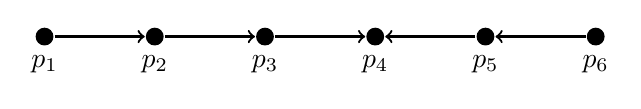
\begin{tikzpicture}
[scale = 0.7,
line width = 0.8pt,
v/.style = {circle, fill = black, inner sep = 0.8mm},u/.style = {circle, fill = white, inner sep = 0.1mm}]
  \node[u] (L1) at (0, -0.5) {$p_1$};
  \node[u] (L1) at (2, -0.5) {$p_2$};
  \node[u] (L1) at (4, -0.5) {$p_3$};
  \node[u] (L1) at (6, -0.5) {$p_4$};
  \node[u] (L1) at (8, -0.5) {$p_5$};
  \node[u] (L1) at (10, -0.5) {$p_6$};
  \node[v] (1) at (0, 0) {};
  \node[v] (2) at (2, 0) {};
  \node[v] (3) at (4, 0) {};
  \node[v] (4) at (6, 0) {};
  \node[v] (5) at (8, 0) {};
  \node[v] (6) at (10, 0) {};  
  \draw[->] (1) to (2);
  \draw[->] (2) to (3); 
  \draw[->] (3) to (4);
  \draw[->] (5) to (4);
  \draw[->] (6) to (5);
\end{tikzpicture}

\end{document}